\chapter{Verkkojen perusteet}

\section{Verkkojen käsitteitä}

Verkko on tietorakenne, joka muodostuu \emph{solmuista} ja
niitä yhdistävistä \emph{kaarista}.
Merkitsemme tässä kirjassa verkon solmujen
määrää kirjaimella $n$ ja verkon kaarten määrää
kirjaimella $m$.
Lisäksi numeroimme yleensä verkon solmut kokonaisluvuin
$1,2,\dots,n$.

Sanomme, että kaksi solmua ovat \emph{vierekkäin} verkossa,
jos niiden välillä on kaari.
Solmun \emph{naapureja} ovat kaikki solmut,
joihin se on yhteydessä kaarella,
ja solmun \emph{aste} on sen naapureiden määrä.
Verkossa oleva \emph{polku} tarkoittaa reittiä
tietystä solmusta toiseen kulkemalla kaaria pitkin.

Kuvassa \ref{fig:veresi} on esimerkkinä verkko,
jossa on 5 solmua ja 7 kaarta.
Solmun 2 aste on 3,
koska sen naapurit ovat solmut 1, 4 ja 5.
Voimme kulkea solmusta 1 solmuun 5 monella tavalla:
mahdollisia polkuja ovat esimerkiksi
$1 \rightarrow 2 \rightarrow 5$ ja
$1 \rightarrow 3 \rightarrow 4 \rightarrow 5$.

\begin{figure}
\center
\begin{center}
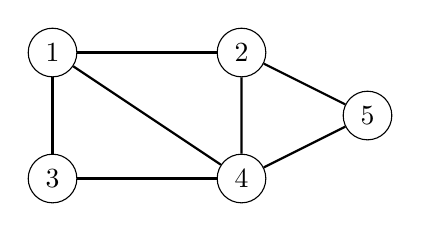
\begin{tikzpicture}[scale=0.8]
\node[draw, circle] (1) at (1,3) {$1$};
\node[draw, circle] (2) at (4,3) {$2$};
\node[draw, circle] (3) at (1,1) {$3$};
\node[draw, circle] (4) at (4,1) {$4$};
\node[draw, circle] (5) at (6,2) {$5$};

\path[draw,thick,-] (1) -- (2);
\path[draw,thick,-] (1) -- (3);
\path[draw,thick,-] (1) -- (4);
\path[draw,thick,-] (3) -- (4);
\path[draw,thick,-] (2) -- (4);
\path[draw,thick,-] (2) -- (5);
\path[draw,thick,-] (4) -- (5);
\end{tikzpicture}
\end{center}
\caption{Verkko, jossa on 5 solmua ja 7 kaarta.}
\label{fig:veresi}
\end{figure}

Verkko on \emph{yhtenäinen}, jos minkä tahansa
kahden solmun välillä on polku.
Esimerkiksi kuvan \ref{fig:veresi} verkko on yhtenäinen.
Jos verkko ei ole yhtenäinen, voimme tarkastella
sen yhtenäisiä \emph{komponentteja}.
Esimerkiksi kuvan \ref{fig:veryht} verkko ei ole yhtenäinen,
ja sen komponentit ovat $\{1,3\}$ ja $\{2,4,5\}$.

\begin{figure}
\center
\begin{center}
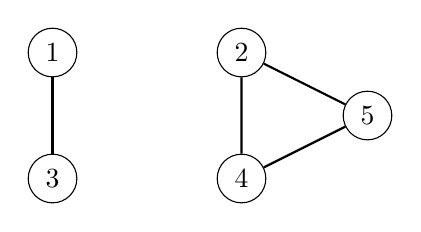
\begin{tikzpicture}[scale=0.8]
\node[draw, circle] (1) at (1,3) {$1$};
\node[draw, circle] (2) at (4,3) {$2$};
\node[draw, circle] (3) at (1,1) {$3$};
\node[draw, circle] (4) at (4,1) {$4$};
\node[draw, circle] (5) at (6,2) {$5$};

\path[draw,thick,-] (1) -- (3);
\path[draw,thick,-] (2) -- (4);
\path[draw,thick,-] (2) -- (5);
\path[draw,thick,-] (4) -- (5);
\end{tikzpicture}
\end{center}
\caption{Verkon yhtenäiset komponentit ovat $\{1,3\}$ ja $\{2,4,5\}$.}
\label{fig:veryht}
\end{figure}

Verkossa oleva \emph{sykli} on polku, jonka ensimmäinen ja viimeinen
solmu on sama.
Esimerkiksi verkossa \ref{fig:veresi} on sykli
$1 \rightarrow 4 \rightarrow 3 \rightarrow 1$.
Verkko on \emph{syklitön}, jos siinä ei ole yhtään sykliä.
Verkko on \emph{puu}, jos se on yhtenäinen ja syklitön.
Puussa kaarten määrä on aina yhden pienempi kuin solmujen määrä.
Esimerkiksi kuvassa \ref{fig:verpuu} on puu, jossa on 5 solmua ja 4 kaarta.

\begin{figure}
\center
\begin{center}
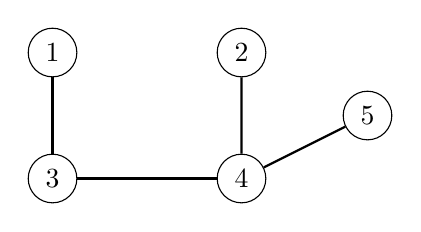
\begin{tikzpicture}[scale=0.8]
\node[draw, circle] (1) at (1,3) {$1$};
\node[draw, circle] (2) at (4,3) {$2$};
\node[draw, circle] (3) at (1,1) {$3$};
\node[draw, circle] (4) at (4,1) {$4$};
\node[draw, circle] (5) at (6,2) {$5$};

\path[draw,thick,-] (1) -- (3);
\path[draw,thick,-] (3) -- (4);
\path[draw,thick,-] (2) -- (4);
\path[draw,thick,-] (4) -- (5);
\end{tikzpicture}
\end{center}
\caption{Puu, jossa on 5 solmua ja 4 kaarta.}
\label{fig:verpuu}
\end{figure}

Verkko on \emph{suunnattu}, jos kaarilla on merkityt suunnat,
joiden mukaisesti niitä on kuljettava.
Kuvassa \ref{fig:versuu} on esimerkkinä suunnattu verkko.
Esimerkiksi voimme kulkea solmusta 1 solmuun 5
polkua $1 \rightarrow 2 \rightarrow 5$,
mutta emme voi kulkea solmusta 5 solmuun 1.

\begin{figure}
\center
\begin{center}
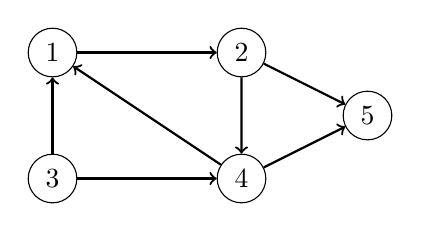
\begin{tikzpicture}[scale=0.8]
\node[draw, circle] (1) at (1,3) {$1$};
\node[draw, circle] (2) at (4,3) {$2$};
\node[draw, circle] (3) at (1,1) {$3$};
\node[draw, circle] (4) at (4,1) {$4$};
\node[draw, circle] (5) at (6,2) {$5$};

\path[draw,thick,->] (1) -- (2);
\path[draw,thick,<-] (1) -- (3);
\path[draw,thick,<-] (1) -- (4);
\path[draw,thick,->] (3) -- (4);
\path[draw,thick,->] (2) -- (4);
\path[draw,thick,->] (2) -- (5);
\path[draw,thick,->] (4) -- (5);
\end{tikzpicture}
\end{center}
\caption{Suunnattu verkko}
\label{fig:versuu}
\end{figure}

Suunnattu verkko on \emph{vahvasti yhtenäinen},
jos verkossa on polku mistä tahansa solmusta
mihin tahansa solmuun.
Esimerkiksi kuvan \ref{fig:versuu} verkko ei
ole vahvasti yhtenäinen,
koska emme voi kulkea solmusta 5 solmuun 1.
Jos verkko ei ole vahvasti yhtenäinen,
voimme jakaa sen vahvasti yhtenäisiin komponentteihin.
Esimerkiksi kuvan \ref{fig:versuu} verkossa
vahvasti yhtenäiset komponentit ovat $\{1,2,4\}$, $\{3\}$ ja $\{5\}$.

Suunnatussa verkossa solmun \emph{lähtöaste} on
solmusta lähtevien kaarten määrä ja solmun \emph{tuloaste}
on solmuun tulevien kaarten määrä.
Esimerkiksi kuvan \ref{fig:versuu} verkossa
solmun 2 lähtöaste on 2 ja tuloaste on 1.

Verkko on \emph{painotettu}, jos sen kaarille on asetettu painot.
Usein painot kuvaavat kaarien pituuksia, ja polun pituus
on siinä olevien painojen summa.
Kuvassa \ref{fig:verpai} on esimerkki painotetusta verkosta.
Esimerkiksi polun $1 \rightarrow 3 \rightarrow 4 \rightarrow 5$
pituus on $2+4+3=9$.

\begin{figure}
\center
\begin{center}
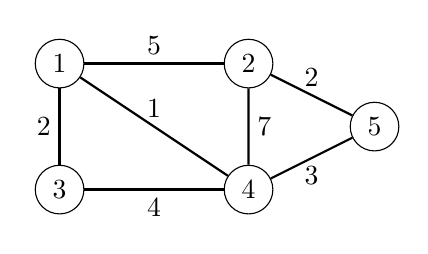
\begin{tikzpicture}[scale=0.8,label distance=-1.5mm]
\node[draw, circle] (1) at (1,3) {$1$};
\node[draw, circle] (2) at (4,3) {$2$};
\node[draw, circle] (3) at (1,1) {$3$};
\node[draw, circle] (4) at (4,1) {$4$};
\node[draw, circle] (5) at (6,2) {$5$};

\path[draw,thick,-] (1) -- node[font=\small,label=above:5] {} (2);
\path[draw,thick,-] (1) -- node[font=\small,label=left:2] {} (3);
\path[draw,thick,-] (1) -- node[font=\small,label=above:1] {} (4);
\path[draw,thick,-] (3) -- node[font=\small,label=below:4] {} (4);
\path[draw,thick,-] (2) -- node[font=\small,label=right:7] {} (4);
\path[draw,thick,-] (2) -- node[font=\small,label=above:2] {} (5);
\path[draw,thick,-] (4) -- node[font=\small,label=below:3] {} (5);
\end{tikzpicture}
\end{center}
\caption{Painotettu verkko}
\label{fig:verpai}
\end{figure}

Verkko on \emph{kaksijakoinen}, jos voimme värittää sen
solmut kahdella värillä niin, että jokaisella
vierekkäisellä solmulla on eri väri.
Esimerkiksi kuvan \ref{fig:verkak} verkko on kaksijakoinen,
koska voimme värittää solmut 1 ja 4 sinisiksi ja
solmut 2, 3 ja 5 punaisiksi.

\begin{figure}
\center
\begin{center}
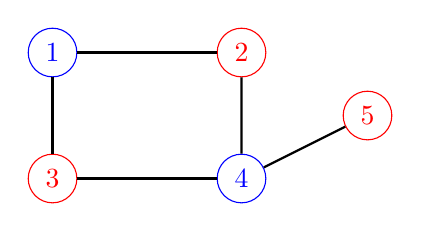
\begin{tikzpicture}[scale=0.8]
\node[draw, circle, color=blue] (1) at (1,3) {$1$};
\node[draw, circle, color=red] (2) at (4,3) {$2$};
\node[draw, circle, color=red] (3) at (1,1) {$3$};
\node[draw, circle, color=blue] (4) at (4,1) {$4$};
\node[draw, circle, color=red] (5) at (6,2) {$5$};

\path[draw,thick,-] (1) -- (2);
\path[draw,thick,-] (1) -- (3);
\path[draw,thick,-] (3) -- (4);
\path[draw,thick,-] (2) -- (4);
\path[draw,thick,-] (4) -- (5);
\end{tikzpicture}
\end{center}
\caption{Kaksijakoinen verkko.}
\label{fig:verkak}
\end{figure}



\section{Verkot ohjelmoinnissa}

\subsection{Vieruslistaesitys}

\subsection{Vierusmatriisiesitys}

\section{Läpikäyntitavat}

\subsection{Syvyyshaku}

\subsection{Leveyshaku}

